% Adapted from Alex Reustle's CMSC351 Course Notes

% This program is free software: you can redistribute it and/or modify
% it under the terms of the GNU General Public License as published by
% the Free Software Foundation, either version 3 of the License, or
% (at your option) any later version.

% This program is distributed in the hope that it will be useful,
% but WITHOUT ANY WARRANTY; without even the implied warranty of
% MERCHANTABILITY or FITNESS FOR A PARTICULAR PURPOSE.  See the
% GNU General Public License for more details.

% You should have received a copy of the GNU General Public License
% along with this program.  If not, see <http://www.gnu.org/licenses/>.
\documentclass[english, 10pt]{article}

\usepackage{notes}
\usepackage{gensymb}
\usepackage{inconsolata}
\usepackage[shellescape]{gmp}
\allowdisplaybreaks%
\newcommand{\thiscoursecode}{CMSC 320}
\newcommand{\thiscoursename}{Introduction to Data Science}
\newcommand{\thisprof}{Prof.\ John Dickerson}
\newcommand{\me}{Akilesh Praveen}
\newcommand{\thisterm}{Fall 2020}
\newcommand{\website}{https://cmsc320.github.io}%chktex 8
\usepackage{ifpdf}
\ifpdf%
\DeclareGraphicsRule{*}{mps}{*}{}
\fi
% \listfiles

\usepackage[utf8]{inputenc}
 
\usepackage{listings}
\lstloadlanguages{Python}
\usepackage{xcolor}
\usetikzlibrary{patterns}
\usepackage[many]{tcolorbox}
 
\definecolor{codegreen}{rgb}{0,0.6,0}
\definecolor{codegray}{rgb}{0.5,0.5,0.5}
\definecolor{codepurple}{rgb}{0.58,0,0.82}
\definecolor{backcolour}{rgb}{0.95,0.95,0.94}
\definecolor{codered}{rgb}{0.5,0.15,0.15}
\definecolor{commentred}{rgb}{1,0.01,0.02}
 
\lstdefinestyle{mystyle}{
    backgroundcolor=\color{backcolour},   
    commentstyle=\color{codegreen},
    keywordstyle=\color{red},
    numberstyle=\tiny\color{codegray},
    stringstyle=\color{codered},
    basicstyle=\ttfamily\footnotesize,
    breakatwhitespace=false,         
    breaklines=true,                 
    captionpos=b,                    
    keepspaces=true,
    xleftmargin=.15\textwidth,
    xrightmargin=.15\textwidth,
    linewidth=\textwidth,                 
    numbers=left,                    
    numbersep=5pt,                  
    showspaces=false,                
    showstringspaces=false,
    showtabs=false,                  
    tabsize=2,
    belowskip=3em,
    aboveskip=3em,
}

\lstset{style=mystyle}


% \VerbEnvir{align tikzpicture algorithm}
%%%Headers
\chead{320 - Intro to Data Science}
\lhead{\thisterm}

%%%%% TITLE %%%%%
\graphicspath{{../}}
\newcommand{\notefront}{%
\pagenumbering{arabic}
\begin{center}
{\small}
\textbf{\Huge{\noun{\thiscoursecode}}}
{\Huge \par}
{\Large{\noun{\thiscoursename}}}\\
\vspace{0.1in}
\vspace{0in}
\includegraphics[scale=0.3]{umd_cs.jpg} \\
\vspace{0.1in}{\noun\me} \\
{\noun\thisprof} \ $\bullet$ \ {\noun\thisterm} \ $\bullet$ \ {\noun{University of Maryland}} \\
{\ttfamily \url{\website}} \\
\end{center}
}

 \tikzstyle{class}=[
    rectangle,
    draw=black,
    text centered,
    anchor=north,
    text=black,
    text width=2cm,
    shading=axis,
    bottom color={rgb:red,222;green,222;blue,222},
    top color=white,shading angle=45]


\newtcolorbox{myproof}[1][]{
   enhanced,arc=0pt, frame hidden, borderline west = {1pt}{0pt}{black}, #1
}

\begin{document}
% \renewcommand\familydefault{\sfdefault}
% \sffamily
  % Notes front
  \notefront%
  % Table of Contents and List of Figures
  \tocandfigures%
  
\section{Notes \& Preface}

Course notes for CMSC320, under Prof. John Dickerson. Notes collected from previous and current lectures.

\section{Lecture 1}

\subsection{What is Data Science?}

Data Science is the application of computation and statistical techniques to address or gain insight.
It's the intersection of statistics and Computer Science.
Based on what I've learned thus far, learning to do data science is like learning how to use a TI-84 in statistics class.
You're simply learning how to leverage programming tools in order to perform advanced, complex, and meaningful data-related operations.\newline

It's the use of statistics and computer science in order to find real-world insights.\newline\newline

{
\centering


\tikzset{every picture/.style={line width=0.75pt}} %set default line width to 0.75pt        

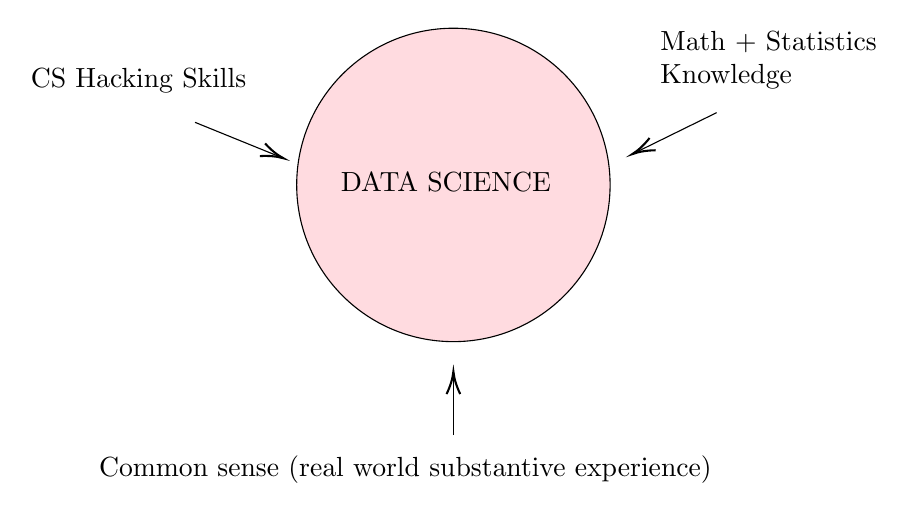
\begin{tikzpicture}[x=0.75pt,y=0.75pt,yscale=-1,xscale=1]
%uncomment if require: \path (0,300); %set diagram left start at 0, and has height of 300

%Shape: Circle [id:dp061140258122834745] 
\draw  [fill={rgb, 255:red, 255; green, 219; blue, 224 }  ,fill opacity=1 ] (254.67,119.5) .. controls (254.67,77.8) and (288.47,44) .. (330.17,44) .. controls (371.86,44) and (405.67,77.8) .. (405.67,119.5) .. controls (405.67,161.2) and (371.86,195) .. (330.17,195) .. controls (288.47,195) and (254.67,161.2) .. (254.67,119.5) -- cycle ;
%Straight Lines [id:da4450208385410075] 
\draw    (205.67,89.33) -- (246.48,105.91) ;
\draw [shift={(248.33,106.67)}, rotate = 202.11] [color={rgb, 255:red, 0; green, 0; blue, 0 }  ][line width=0.75]    (10.93,-3.29) .. controls (6.95,-1.4) and (3.31,-0.3) .. (0,0) .. controls (3.31,0.3) and (6.95,1.4) .. (10.93,3.29)   ;
%Straight Lines [id:da055339322100053545] 
\draw    (457,84.67) -- (418.13,103.78) ;
\draw [shift={(416.33,104.67)}, rotate = 333.81] [color={rgb, 255:red, 0; green, 0; blue, 0 }  ][line width=0.75]    (10.93,-3.29) .. controls (6.95,-1.4) and (3.31,-0.3) .. (0,0) .. controls (3.31,0.3) and (6.95,1.4) .. (10.93,3.29)   ;
%Straight Lines [id:da5012858238681945] 
\draw    (330.17,240) -- (330.17,211.33) ;
\draw [shift={(330.17,209.33)}, rotate = 450] [color={rgb, 255:red, 0; green, 0; blue, 0 }  ][line width=0.75]    (10.93,-3.29) .. controls (6.95,-1.4) and (3.31,-0.3) .. (0,0) .. controls (3.31,0.3) and (6.95,1.4) .. (10.93,3.29)   ;

% Text Node
\draw (274.67,112.5) node [anchor=north west][inner sep=0.75pt]   [align=left] {DATA SCIENCE};
% Text Node
\draw (125.33,62) node [anchor=north west][inner sep=0.75pt]   [align=left] {CS Hacking Skills};
% Text Node
\draw (428.67,44.33) node [anchor=north west][inner sep=0.75pt]   [align=left] {Math + Statistics\\Knowledge};
% Text Node
\draw (158.17,248.67) node [anchor=north west][inner sep=0.75pt]   [align=left] {Common sense (real world substantive experience)};


\end{tikzpicture}

}

\subsection{Topics}

Here are the general topics that this class will cover.

\begin{itemize}
	\item Processing data
	\item Visualizing data
	\item Understanding data
	\item Communicating data
	\item Extracting value from data
\end{itemize}

\subsection{Tools}

Here are some tools commonly employed by data scientists. We'll try to cover how to use most of them here.

\begin{itemize}
	\item Python
	\item Scikit-Learn
	\item Docker
	\item PANDAS
	\item Spark
	\item TensorFlow
\end{itemize}

\subsection{Conda}

Conda is a package and environment manager for python that we can use with the command line.
We can create multiple environments for us and install separate packages in each of them.
This will be highly useful to us, as we sometimes want to consolidate the tools we use into separate environments.

\section{Lecture 2}

\begin{tcolorbox}[title=Definition:,colframe=red!75!black,colback=red!5!white,arc=0pt,fonttitle=\bfseries]
\textbf{Data Collection} $\rightarrow$ The process of measuring and gathering information on targeted variables.
\end{tcolorbox}

\subsection{Literate Programming}

The idea of \textbf{literate programming} is that you have the source code, an explanation of the source code, and the end result of running the code all in one file. Usually, this file is identified as a \textit{notebook}. In other words, the syntax is no different from regular code, you just get a more organized way to show off tables, plots, and other outputs generated from your code.

\subsection{Jupyter Notebook + Alternatives}

Jupyter Notebook is a service that started off as \texttt{iPython}, but it's basically a web-based platform that we use for literate programming. Specifically, it supports Python-based literate programming. Most data scientists prefer it, and it can also apparently leverage big data tools, such as Apache Spark.\newline

It saves files in \texttt{.ipynb} format, which most platforms (i.e. GitHub) have built in viewers for. Options to export in other readable formats are available. Basically, it's just Python with a bunch of bells and whistles on top to make the output of your code look pretty.\newline

\textit{Apache Zeppelin} is an alternative data analysis tool, but we will stick to Jupyter for our purposes. This is because Jupyter seems to be preferred in industry.\newline

\textit{RStudio} is the equivalent, for people who prefer to use the \texttt{R} programming language for data science.\newline

This course will be centered around Jupyter Notebook.

\subsection{List Comprehensions in Python}

To make lists in Python, you can use loops or the \texttt{map()} function, but a \textit{pythonic} way of doing this would be to use a list comprehension. Below is a simple example.\newline

\begin{myproof}
\textbf{Example:} Make a list of all the squares of \texttt{\{0,1,2,3,4,5,6,7,8,9\}}\newline\newline
\textbf{List Comprehension:}\newline
\texttt{squares = [i * i for i in range(10)]}
\end{myproof}

A good way of thinking about this is that it allows you to build sets like a mathematician. This is a common theme in data science, where we can find the intersection between a lot of math stuff and computer science stuff. It's good to know how lists are generated in a mathematical sense in Python for that reason. Here's an example where we translate mathematical notation into a Python list comprehension.\\

\begin{myproof}
\textbf{Example:} Make a list of all odd natural numbers from 0 to 999\\\\
\textbf{Math Notation:}\\ $E =$ \{$x$ | $x$ in $\mathbb{N} \land x$ is odd $\land x<1000$ \}\\\\
\textbf{List Comprehension:}\\
\texttt{E = [x for x in range(1000) if x \% 2 != 0]}
\end{myproof}

\subsection{Using Python3}

We will use Python3. Since I used Python2 during my internship, I'm going to note some big changes to keep track of.\\

\begin{itemize}
	\item Python3 is backwards incompatible. (Don't write in Python2!)
	\item Print has changed from a command to a function, so make sure to use proper function notation when invoking it.
	\item Division has changed. \texttt{1/2} no longer equals 0. \texttt{1/2 == 0.5} and floored division is now taken care of this way: \texttt{1//2 == 0}
\end{itemize}

\subsection{Python vs. R for Data Scientists}

Some arguments for both sides in terms of what to use.

\begin{itemize}
	\item Python is a 'full' programming langauge. Also, if you've got prior experience with Python paradigms or just programming in general, that's a big plus in terms of learning curve.
	\item R has more mature 'pure statistics' libraries, but Python is apparently catching up.
	\item In terms of \textbf{processing speed}, R is certainly faster. It was designed and optimized for statistics processing.
	\item Python is preferable for machine learning operations, which is pretty big right now.
\end{itemize}

My personal choice will be to use Python as much as I can when I'm studying this course. Since it's more prominent in the tech industry, I should be using it more anyway.

\subsection{The Classic Statistical View of Data}

There are \textbf{four} main types of data: Nominal, Ordinal, Interval, and Ratio data. They can each be classified under two main subgroups, Categorical and Numerical data. Here's a visualization.\\

{
\centering



\tikzset{every picture/.style={line width=0.75pt}} %set default line width to 0.75pt        

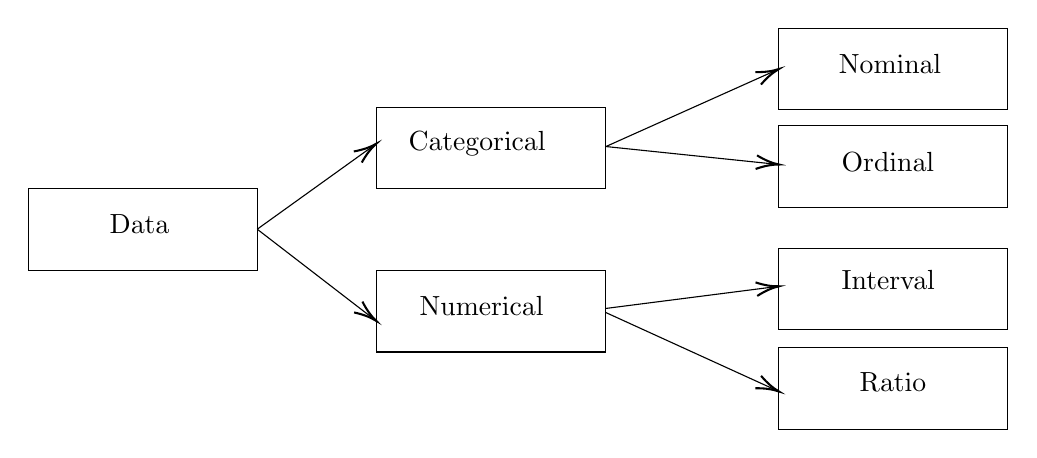
\begin{tikzpicture}[x=0.75pt,y=0.75pt,yscale=-1,xscale=1]
%uncomment if require: \path (0,300); %set diagram left start at 0, and has height of 300

%Shape: Rectangle [id:dp8149613399348021] 
\draw   (72,131) -- (182.33,131) -- (182.33,170.33) -- (72,170.33) -- cycle ;
%Shape: Rectangle [id:dp680618887900226] 
\draw   (239.67,91.67) -- (350,91.67) -- (350,131) -- (239.67,131) -- cycle ;
%Shape: Rectangle [id:dp777477779359951] 
\draw   (239.67,170.33) -- (350,170.33) -- (350,209.67) -- (239.67,209.67) -- cycle ;
%Shape: Rectangle [id:dp9580214955547155] 
\draw   (433.67,53.67) -- (544,53.67) -- (544,93) -- (433.67,93) -- cycle ;
%Shape: Rectangle [id:dp19525566557447283] 
\draw   (433.67,100.5) -- (544,100.5) -- (544,139.83) -- (433.67,139.83) -- cycle ;
%Shape: Rectangle [id:dp18958725273981114] 
\draw   (433.67,159.67) -- (544,159.67) -- (544,199) -- (433.67,199) -- cycle ;
%Shape: Rectangle [id:dp27616820331988945] 
\draw   (433.67,207.67) -- (544,207.67) -- (544,247) -- (433.67,247) -- cycle ;
%Straight Lines [id:da07504069427898741] 
\draw    (182.33,150.5) -- (238.04,110.5) ;
\draw [shift={(239.67,109.33)}, rotate = 504.32] [color={rgb, 255:red, 0; green, 0; blue, 0 }  ][line width=0.75]    (10.93,-3.29) .. controls (6.95,-1.4) and (3.31,-0.3) .. (0,0) .. controls (3.31,0.3) and (6.95,1.4) .. (10.93,3.29)   ;
%Straight Lines [id:da18494381831895634] 
\draw    (182.33,150.5) -- (238.08,193.45) ;
\draw [shift={(239.67,194.67)}, rotate = 217.61] [color={rgb, 255:red, 0; green, 0; blue, 0 }  ][line width=0.75]    (10.93,-3.29) .. controls (6.95,-1.4) and (3.31,-0.3) .. (0,0) .. controls (3.31,0.3) and (6.95,1.4) .. (10.93,3.29)   ;
%Straight Lines [id:da49166239871511697] 
\draw    (350.33,110.67) -- (431.84,74.15) ;
\draw [shift={(433.67,73.33)}, rotate = 515.87] [color={rgb, 255:red, 0; green, 0; blue, 0 }  ][line width=0.75]    (10.93,-3.29) .. controls (6.95,-1.4) and (3.31,-0.3) .. (0,0) .. controls (3.31,0.3) and (6.95,1.4) .. (10.93,3.29)   ;
%Straight Lines [id:da6935259459415319] 
\draw    (350.33,110.67) -- (431.68,119.13) ;
\draw [shift={(433.67,119.33)}, rotate = 185.94] [color={rgb, 255:red, 0; green, 0; blue, 0 }  ][line width=0.75]    (10.93,-3.29) .. controls (6.95,-1.4) and (3.31,-0.3) .. (0,0) .. controls (3.31,0.3) and (6.95,1.4) .. (10.93,3.29)   ;
%Straight Lines [id:da6050313931467277] 
\draw    (350.33,190.67) -- (431.85,227.84) ;
\draw [shift={(433.67,228.67)}, rotate = 204.51] [color={rgb, 255:red, 0; green, 0; blue, 0 }  ][line width=0.75]    (10.93,-3.29) .. controls (6.95,-1.4) and (3.31,-0.3) .. (0,0) .. controls (3.31,0.3) and (6.95,1.4) .. (10.93,3.29)   ;
%Straight Lines [id:da8985137963347964] 
\draw    (350.33,188.67) -- (431.68,178.25) ;
\draw [shift={(433.67,178)}, rotate = 532.71] [color={rgb, 255:red, 0; green, 0; blue, 0 }  ][line width=0.75]    (10.93,-3.29) .. controls (6.95,-1.4) and (3.31,-0.3) .. (0,0) .. controls (3.31,0.3) and (6.95,1.4) .. (10.93,3.29)   ;

% Text Node
\draw (110,142.17) node [anchor=north west][inner sep=0.75pt]   [align=left] {Data};
% Text Node
\draw (254,102) node [anchor=north west][inner sep=0.75pt]   [align=left] {Categorical};
% Text Node
\draw (259.33,181.33) node [anchor=north west][inner sep=0.75pt]   [align=left] {Numerical};
% Text Node
\draw (461.33,65) node [anchor=north west][inner sep=0.75pt]   [align=left] {Nominal};
% Text Node
\draw (462.67,112) node [anchor=north west][inner sep=0.75pt]   [align=left] {Ordinal};
% Text Node
\draw (462.67,168.83) node [anchor=north west][inner sep=0.75pt]   [align=left] {Interval};
% Text Node
\draw (471.33,218.33) node [anchor=north west][inner sep=0.75pt]   [align=left] {Ratio};


\end{tikzpicture} \\
}

\subsubsection{Nominal Data}

A type of categorical data, nominal data value have names and describe the state of things. For example, your marriage status is nominal data because you can either be \textit{single}, \textit{married}, or \textit{separated}. Another example is the type of drink you're going to have. Will it be \textit{Milk}, \textit{Beer}, or \textit{Juice}?\\

The key here is that there can be no quantitative values assigned to each of these categories, as that would allow us to do math with them and would defeat the purpose of these labels. These values \textbf{cannot be easily compared}, so they have no material value. \textit{E.g. being single is not quantitatively better than being married (objectively), and vice versa}.\\

\begin{myproof}
\textbf{Example:} What is your marital status?
\begin{itemize}
	\item Married
	\item Divorced (separated)
	\item Single
\end{itemize}
\end{myproof}

\subsubsection{Ordinal Data}

Ordinal data represents values that have names that describe the state of things, but in this case, there \textbf{is} an ordering of those values. This is what sets it apart from nominal data. \\ 
\begin{myproof}
\textbf{Example:} What did you think of the movie?
\begin{itemize}
	\item Strongly liked
	\item Liked
	\item Indifferent
	\item Disliked
	\item Strongly Disliked
\end{itemize}
\end{myproof}

Given how subjective some of these things can be, the distinction between nominal and ordinal can be \textbf{blurry} at times. For example, going back to our nominal example, some people may think that being single is quantitatively better than being married.

\subsubsection{Interval and Ratio Data}

Interval and Ratio data are pretty similar, and both can be used to measure things that can be represented by either integers or real numbers. \\

\textbf{Interval} data scales with fixed but arbitrary values. That might sound silly, but a good example is \textbf{dates}. Below is an example of two data comparisons of interval data that seem arbitrary, but indeed hold integer value.\\

\begin{myproof}
\textbf{Example:} The following two operations are equal. \\\\
\texttt{10/1/2019 - 9/1/2019} \\
\texttt{10/1/2018 - 9/1/2018}
\end{myproof}

The measures don't look like integer values at first, but we can quantify them by marking them with days.\\

Here's what sets \textbf{Interval} data apart, however. You have \textbf{no method} of computing ratios or scales with it. For example, never mind that you can try computing \texttt{(9/1/2019 $\times$ 8/25/2015)}, the unit of the answer would be totally useless to us, and neither would the actual number, even if you went ahead with the operation.\\

\textbf{Ratio} data is, in essence, the same as interval data in that it is numerical, but the scale itself \textbf{has a true zero}. While dates don't necessarily have a true zero, we can say that money counts as ratio data. For example, having zero money means that you're at the absolute zero of that scale, whereas the absolute zero for dates is disputable. Are we saying we're starting at O A.D.? The Big Bang? Even earlier?\\

Differentiating between the two is usually a case-by-case basis thing, which is what I'm thinking is the best way to handle any conflicts I end up running into between ratio and interval data.\\

\begin{myproof}
\textbf{Example:} Interval data \\\\
Temperature on the scale of Celsius or Fahrenheit is interval-type data because $0\degree$ is set to an arbitrarily fixed point. Also, we can't scale it properly- $30\degree F$ isn't twice as hot as $15\degree F$.\\\\
\textbf{Example:} Ratio data \\\\
Temperature on the Kelvin scale is ratio data. $0K$ is set at legitimate absolute zero, and $50K$ is truly twice as cold as $100K$.
\end{myproof}

\subsection{Data Science at a Glance}

Data science is basically manipulating and computing using data. As such, we need to shift our thinking from writing \textbf{imperative} code to manipulate \textbf{data structures} to creating \textbf{sequences and pipelines} to conduct operations on \textbf{data}. That stuff is covered more in 420 and 424, for reference.\newline

More often than not, we have to take the data that we've found and make it easily understandable for humans. This is called Data Representation.\newline

\begin{tcolorbox}[title=Definition:,colframe=red!75!black,colback=red!5!white,arc=0pt,fonttitle=\bfseries]
\textbf{Data Representation} $\rightarrow$ The natural way to think about data, in a human way.
\end{tcolorbox}

Here are some ways that we think about data in this class:\newline

\begin{itemize}
	\item \textbf{One Dimensional Arrays} $\rightarrow$ E.g. \texttt{<'red', 'blue', 'green'>} or \texttt{<0,3,4>}. We can use functions like map, fold and filter to manipulate these.
	\item \textbf{N-Dimensional Arrays} $\rightarrow$ Also known as \textbf{tensors}.
	\begin{itemize}
		\item For example, a Tensor of dimensions \texttt{[6,4]} is just a $6\times 4$ matrix.
		\item Similarly, a Tensor of dimensions \texttt{[4,4,2]} is a 3D array.
		\item Here, we can start to make use of \textbf{Linear Algebra} for further data manipulation. Some example operations that we can use to mess with tensors:
		\begin{itemize}
			\item Matrix/Tensor Multiplications
			\item Transpose
			\item Vector Multiplication
			\item Matrix Factorization (we will explore this later)
		\end{itemize}
	\end{itemize}
	\item \textbf{Sets} of objects, or \textbf{Key/Value Pairs}
	\item \textbf{Tables/Relations} $\rightarrow$ This goes into relational databases, which is the basis of \texttt{SQL}. We'll go into this later.
	\item \textbf{Hierarchies/Trees/Graphs} $\rightarrow$ This sort of spills over into data structures, but they've got some additional nuances included with them.
	\begin{itemize}
		\item They tend to make use of 'path' queries
		\item Graph and Tree Algorithms will be useful here, efficiency is key
		\item Example: networks are represented this way, we'll cover that later in this class
	\end{itemize}
\end{itemize}

\section{Lecture 3}

\subsection{Acquiring Data}

Here are some examples of how we can grab data from places. Pretty obvious, common sense stuff. We're going to explore all of these as we move forward.

\begin{itemize}
	\item Direct download from online or loading it from local storage
	\item Generate the data locally via a simulation or equivalent program
	\item Query data from a database 
	\item Query data from an API
	\item Scrape data from a website
\end{itemize}

When you pull from APIs, you're going to want to be using HTTP Requests.

\subsection{RESTful APIs}

This stands for REpresentational State Transfer APIs, and it's basically a standard that enforces that APIs do a few things. It says that they should support these basic operations:

\begin{itemize}
	\item \texttt{GET} $\rightarrow$ Query a data entry
	\item \texttt{POST} $\rightarrow$ Create a new data entry
	\item \texttt{PUT} $\rightarrow$ Update an existing data entry
	\item \texttt{DELETE} $\rightarrow$ Delete an existing data entry
\end{itemize}

RESTful APIs are also supposed to be stateless. That is, with every API request, you send a token of who you are, and you get a current capture of the data at that time/edit the data.\newline

A good example of a REST API is Github, where you can use REST API calls on your repositories.\newline

There are other guiding principles and miscellaneous guidelines for RESTful APIs, which can all be found at \texttt{https:/restfulapi.net}\newline

\begin{tcolorbox}[title=Aside: GRAPHQL,colframe=black,colback=white,arc=0pt,fonttitle=\bfseries]
\textbf{GraphQL} $\rightarrow$ REST has been adopted by many developers and is widely regarded as the traditional way to send data over HTTP. GraphQL, on the other hand, is a revolutionary new player that's presented as a way to \textit{replace} legacy REST APIs \textit{(back4apps)}
\end{tcolorbox}

\subsection{Oauth}

If you want to grant an app access to your identity without actually giving it your username and password, is there a way to do that? The answer is \textbf{yes}, because this is a common software engineering problem.\newline

\textbf{OAuth} is the standard for \textit{access delegation} used for internet users to grant websites access to their information on other sites. A pretty good example of this is Google's sign in page on other websites. How do you think other websites conduct sign in without knowing your password for your Google account?

\subsection{GET Requests}

Assume we used Python's \texttt{requests} module to query a server with a \texttt{GET} request.\newline

First, we'd get either a \texttt{CSV}, \texttt{JSON}, or \texttt{HTML/XML/XHTML} file back, in response. This is the data that we have to sift through. \textit{Note:} You might also get a domain-specific file, like an \textbf{rvt} file. You're always welcome to make your own filetype for storing data, but make sure it's actually documented somewhere.\newline

\begin{tcolorbox}[title=Aside: Parsing CSVs and JSON,colframe=black,colback=white,arc=0pt,fonttitle=\bfseries]
Never write your own \texttt{CSV} or \texttt{JSON} parsers. This is another example of reinventing the wheel. We'll use Python Libraries to do this more easily. \textit{E.g. PANDAS}
\end{tcolorbox}

\subsection{More on Data Storage Formats}

\begin{tcolorbox}[title=Definition:,colframe=red!75!black,colback=red!5!white,arc=0pt,fonttitle=\bfseries]
\textbf{Serialization} $\rightarrow$ The process of converting objects into strings.\newline
\textbf{Deserialization} $\rightarrow$ The process of converting strings back into objects.
\end{tcolorbox}

\textbf{\texttt{JSON}} is a pretty common format for serializing objects. Plus, serializing objects makes it easier for humans to read and perform sanity-checks on. In Python, \texttt{JSON} is built with Strings, Lists, Dictionaries, and sometimes mixes of a few of those together.\newline

\begin{tcolorbox}[title=Definition:,colframe=red!75!black,colback=red!5!white,arc=0pt,fonttitle=\bfseries]
\textbf{Document Object Model} $\rightarrow$ A tree-based data storage method. For example, HTML is structured this way.
\end{tcolorbox}

\subsubsection{SAX}

SAX is a lightweight way to process XML. It generates a stream of events as it parses an XML file. IT helps us pay attention to individual parts of an XML file without having to process through the rest of it.

\subsection{Parsing HTML}

Parsing HTML is the hardest to do in this case, as I've seen many times before in hackathon projects. Although HTML's specifications are pure, the real world examples of it are pretty nightmarish, thanks to how it interacts with JavaScript and loads dynamic content. All in all, it's fairly unreliable in terms of parsing it manually.\newline

In this case, we're best off using the Python library \texttt{BeautifulSoup}. We can also make use of Python's Regex, which is similar enough to Ruby regex that we worked with in 330. A website like Rubular-\texttt{https://pythex.org} will be useful in this case.\newline

By combining \texttt{BeautifulSoup}, Regular expressions, and \texttt{GET} requests, we can make the process fairly streamlined. This is usually what we'll be using to scrape websites. In order to scrape more dynamic websites, we'd probably have to make use of Selenium. Check my 320 folder to find an example of a simple webscraper with \texttt{BeautifulSoup}.

\section{Lecture 4}

\textbf{Overview:} \textbf{Numpy, PANDAS, Relational Databases, Apache Spark}\newline

\subsection{Available Technologies}

Python has a bunch of 3rd party packages for scientific and numerical computation. Some examples are..

\begin{itemize}
	\item \textbf{\texttt{Numpy} and \texttt{Scipy}} $\rightarrow$ Numerical and scientific function libraries.
	\item \textbf{\texttt{NUMBA}} $\rightarrow$ A Python compiler supporting 'Just in Time' compilation. That is, it supports compilation of code while code is running.
	\item \textbf{\texttt{ALGLIB}} $\rightarrow$ A cross-platform numerical analysis library
	\item \textbf{\texttt{PANDAS}} $\rightarrow$ An extensive data analysis tool with some neat built-in data structures
	\item \textbf{\texttt{PyGSL}} $\rightarrow$ GNU Scientific Library in Python
	\item \textbf{Scientific Python} $\rightarrow$ A collection of scientific computing modules for Python
\end{itemize}

These are a bunch of examples of what's available to developers right now, but we won't focus on all of it. Particular emphasis will be placed on \texttt{Numpy} and \texttt{PANDAS}.

\subsection{NumPy Stack}

The \textbf{NumPy} stack is the most commonly used out of all of these packages. It includes the following:

\begin{itemize}
	\item \texttt{Numpy} - Works sort of like MatLab, just lets us handle a lot of number manipulation and mathematical operations
	\item \texttt{Matplotlib} - This is a plotting and graphing library
	\item \texttt{PANDAS} - This gives us a bunch of data structures and data analysis tools to play with/keep track of our data. (Usually, you'll want to import your data into a \texttt{PANDAS} \texttt{dataframe} or something.)
	\item \texttt{SciPy}
	\item \texttt{SymPy}
	\item \texttt{Jupyter} - This will be our medium for \textbf{literate programming}.
\end{itemize}

To see more about this stuff, search Google for the \textbf{NumPy Stack} and you'll find everything you need.

\subsubsection{Misc About NumPy}

Here are a few more notable things about \texttt{Numpy}:

\begin{itemize}
	\item It contains the \textbf{n-dimensional array} object
	\item It contains 'sophisticated' functions that we can use
	\item It provides us with excellent tools to integrate \texttt{C++}, \texttt{C}, and even \texttt{FORTRAN}
	\item It has math capabilities that are highly useful to us (e.g. Linear Algebra, Fourier Transform, etc)
	\item \texttt{Numpy} also comes with a bunch of new DataTypes for us to use.
\end{itemize}

\begin{tcolorbox}[title=Aside: Numpy Arrays,colframe=black,colback=white,arc=0pt,fonttitle=\bfseries]
Arrays in \texttt{Numpy} are different from regular lists in Python, so make sure your syntax is correct and you know the difference when you decide to use either one in practice.
\end{tcolorbox}

\subsubsection{Linear Algebra with NumPy}

One of \texttt{NumPy}'s most common uses lies within its \textbf{Linear Algebra} module. It allows us to do regular LA stuff, like \texttt{.transpose()} and \texttt{.inverse()} to matrices stored as n-dim arrays. Here's an example.

{\centering
\begin{lstlisting}[language=python]
# Note: remember, we have to use NumPy's n-dimensional array object here

array([[1.0, 2.0],
       [3.0, 4.0]]).transpose()
\end{lstlisting}
}

\subsubsection{SciPy}

\textbf{\texttt{SciPy}} includes various tools and functions for solving common problems in \textbf{scientific computing}.\\

We won't use it much for now, but it's supposed to be good to know. Often you'll be able to find higher-level \texttt{Scipy} functions that will work around the need to call lower-level \texttt{Scipy} functions. It's got a lot of functionality built in, so make sure not to overlook it.

\subsection{The Idea of Reproducibility}

Starting from the same dataset, can we reproduce your analysis and get the same results? \textbf{This is the goal that we're trying to fulfill with our analysis}- we want our stuff to be reproducible! (Otherwise, what exactly does it even mean?)

\subsection{Best Practices}

Honestly, most of this stuff should be common sense.

\begin{itemize}
	\item Use version control to keep track of code. (e.g. \texttt{git})
	\item Use unit testing. (e.g. \texttt{unittest} module in python)
	\item Use libraries when you can. (don't reinvent the wheel!)
\end{itemize}

\subsection{The Idea of Open Data}

Some data should be widely available for everyone to use as they want, without restrictions from copyright, etc.\\

This is probably where all of our free data comes from, so this idea is super helpful to us as data scientists.

\subsection{General Process}

Here's the general process for data science- just so we have an idea of what's going on.\\



\tikzset{every picture/.style={line width=0.75pt}} %set default line width to 0.75pt        

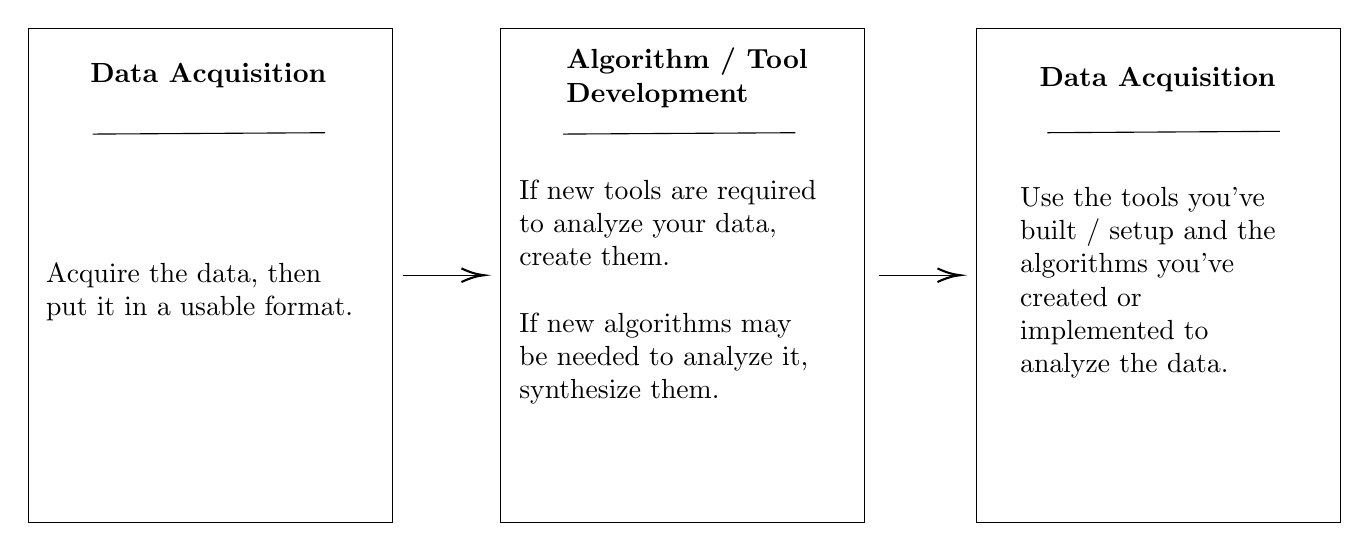
\begin{tikzpicture}[x=0.75pt,y=0.75pt,yscale=-1,xscale=1]
%uncomment if require: \path (0,300); %set diagram left start at 0, and has height of 300

%Shape: Rectangle [id:dp9523245055647409] 
\draw   (34.67,19.33) -- (210.33,19.33) -- (210.33,257.33) -- (34.67,257.33) -- cycle ;
%Shape: Rectangle [id:dp26296611780141976] 
\draw   (262,19.33) -- (437.67,19.33) -- (437.67,257.33) -- (262,257.33) -- cycle ;
%Shape: Rectangle [id:dp4749898829673477] 
\draw   (491.33,19.33) -- (667,19.33) -- (667,257.33) -- (491.33,257.33) -- cycle ;
%Straight Lines [id:da3772898435405757] 
\draw    (65.67,70.33) -- (177.67,69.67) ;
%Straight Lines [id:da47086799536926727] 
\draw    (292.33,70.33) -- (404.33,69.67) ;
%Straight Lines [id:da16258158592667293] 
\draw    (525.67,69.67) -- (637.67,69) ;
%Straight Lines [id:da8259565971285442] 
\draw    (215,138.33) -- (252.33,138.33) ;
\draw [shift={(254.33,138.33)}, rotate = 180] [color={rgb, 255:red, 0; green, 0; blue, 0 }  ][line width=0.75]    (10.93,-3.29) .. controls (6.95,-1.4) and (3.31,-0.3) .. (0,0) .. controls (3.31,0.3) and (6.95,1.4) .. (10.93,3.29)   ;
%Straight Lines [id:da6335608206253658] 
\draw    (444.33,138.33) -- (481.67,138.33) ;
\draw [shift={(483.67,138.33)}, rotate = 180] [color={rgb, 255:red, 0; green, 0; blue, 0 }  ][line width=0.75]    (10.93,-3.29) .. controls (6.95,-1.4) and (3.31,-0.3) .. (0,0) .. controls (3.31,0.3) and (6.95,1.4) .. (10.93,3.29)   ;

% Text Node
\draw (63.33,35) node [anchor=north west][inner sep=0.75pt]   [align=left] {\textbf{Data Acquisition}};
% Text Node
\draw (292.67,27.67) node [anchor=north west][inner sep=0.75pt]   [align=left] {\textbf{Algorithm / Tool}\\\textbf{Development}};
% Text Node
\draw (520.67,37) node [anchor=north west][inner sep=0.75pt]   [align=left] {\textbf{Data Acquisition}};
% Text Node
\draw (42,131.33) node [anchor=north west][inner sep=0.75pt]   [align=left] {Acquire the data, then\\put it in a usable format.};
% Text Node
\draw (270,91.33) node [anchor=north west][inner sep=0.75pt]   [align=left] {If new tools are required\\to analyze your data,\\create them.\\\\If new algorithms may\\be needed to analyze it,\\synthesize them.};
% Text Node
\draw (511.33,94.67) node [anchor=north west][inner sep=0.75pt]   [align=left] {Use the tools you've\\built / setup and the \\algorithms you've \\created or \\implemented to \\analyze the data.};


\end{tikzpicture}

\hfill \break After we do that, we still technically have some programming left. In this new era of literate programming, there's one more step of processing we have to do with our results in order to make them publicly presentable and meaningful.\\



\tikzset{every picture/.style={line width=0.75pt}} %set default line width to 0.75pt        

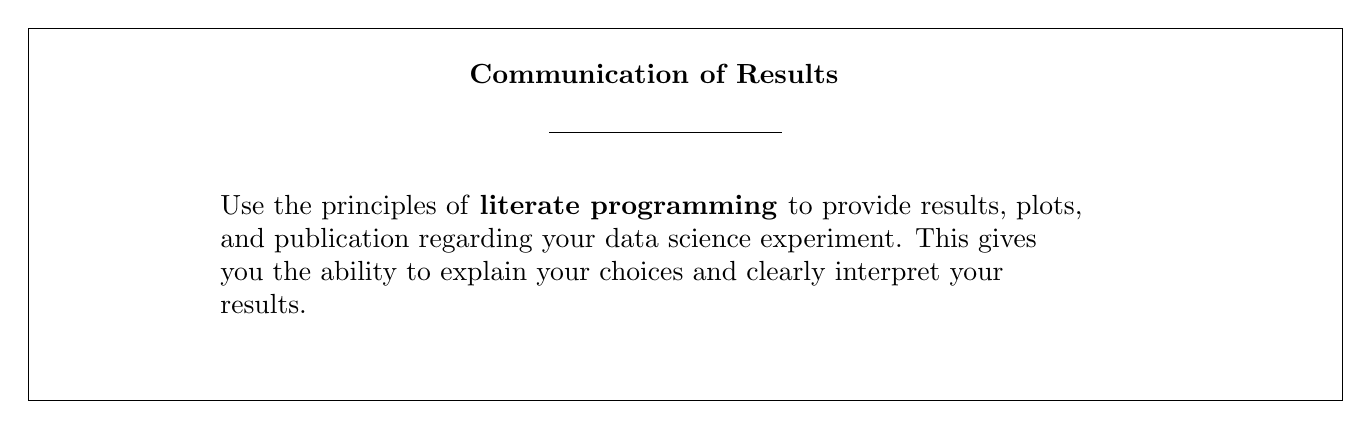
\begin{tikzpicture}[x=0.75pt,y=0.75pt,yscale=-1,xscale=1]
%uncomment if require: \path (0,300); %set diagram left start at 0, and has height of 300

%Shape: Rectangle [id:dp9523245055647409] 
\draw   (34.67,19.33) -- (667.67,19.33) -- (667.67,198.67) -- (34.67,198.67) -- cycle ;
%Straight Lines [id:da3772898435405757] 
\draw    (285.67,69.67) -- (397.67,69.67) ;

% Text Node
\draw (246,35.67) node [anchor=north west][inner sep=0.75pt]   [align=left] {\textbf{Communication of Results}};
% Text Node
\draw (126,98.33) node [anchor=north west][inner sep=0.75pt]   [align=left] {Use the principles of \textbf{literate programming }to provide results, plots,\\and publication regarding your data science experiment. This gives\\you the ability to explain your choices and clearly interpret your\\results.};


\end{tikzpicture}


\hfill \break It's emphasized a lot here to think like an \textbf{algorithm developer}, as you're going to need efficiency in the data analysis that you perform. However, you also need to think like an experiment-conducting \textbf{data scientist}. We don't usually get enough training as the latter, so hopefully this course should be an introduction to that sort of stuff.

\subsection{Project Organization}

Make sure to organize your project in folders appropriately. Specifically, even if you have a lot of components, group with with a focus on experimental procedure.\\

You should certainly be isolating things like \textbf{data}, \textbf{tools}, and \textbf{experiments} into their own folders. Data could include your raw input data, along with data that you've done some processing on. Tools could include Python environment you're using, and experiments could include the meat of what your data science work will be- pipeline scripts, results, figures, plots, analysis scripts, etc.

\subsection{A Little on Bias, Ethics, Responsibility}

\begin{tcolorbox}[title=Aside: Fairness Through Blindness,colframe=black,colback=white,arc=0pt,fonttitle=\bfseries]
The concept of not letting an algorithm look at protected attributes in order to keep it from forming potentially harmful biases.
\end{tcolorbox}

\hfill \break A great example of fairness through blindness could be software that determines the outcome for a loan application. We want the results to be \textbf{independent} of an applicant's race, but they can be \textbf{dependent} on non-protected attributes, such as credit history and income.\\

\begin{tcolorbox}[title=Aside: FATML,colframe=black,colback=white,arc=0pt,fonttitle=\bfseries]
\textbf{FATML} stands for Fairness, Accountability, and Transparency in Machine Learning.
\end{tcolorbox}

\hfill \break Overall, here are some guiding principles for data ethics:

\begin{itemize}
	\item Start with clear user need, with a focus on public benefit. (Can't go wrong with this!)
	\item Use data and tools that emphasize \textbf{minimum} intrusion/invasion of privacy. (Sometimes, we have no choice but to handle sensitive data)
	\item Create robust data science models that minimize bias and focus on objective accuracy.
	\item Be alert to public perceptions.
	\item Be open and accountable for your actions.
	\item Security is key- especially if working with sensitive data.
\end{itemize}

\section{Lecture 5 \& 6}

\textbf{Big ideas: Pandas + Relational Databases}

\begin{itemize}
	\item Tables (Specifically, the abstraction + operations)
	\item \texttt{PANDAS}
	\item The idea of 'tidy' data
	\item \texttt{SQL}
\end{itemize}

\subsection{Tables}

Here's the idea- we can abstract data into our own little data structures just like computer scientists do, and a lot of the time, in data science, tables are the optimal way to do that. (This is why software like PANDAS and Numpy have excellent support for these structures.)\\

{
\centering



\tikzset{every picture/.style={line width=0.75pt}} %set default line width to 0.75pt        

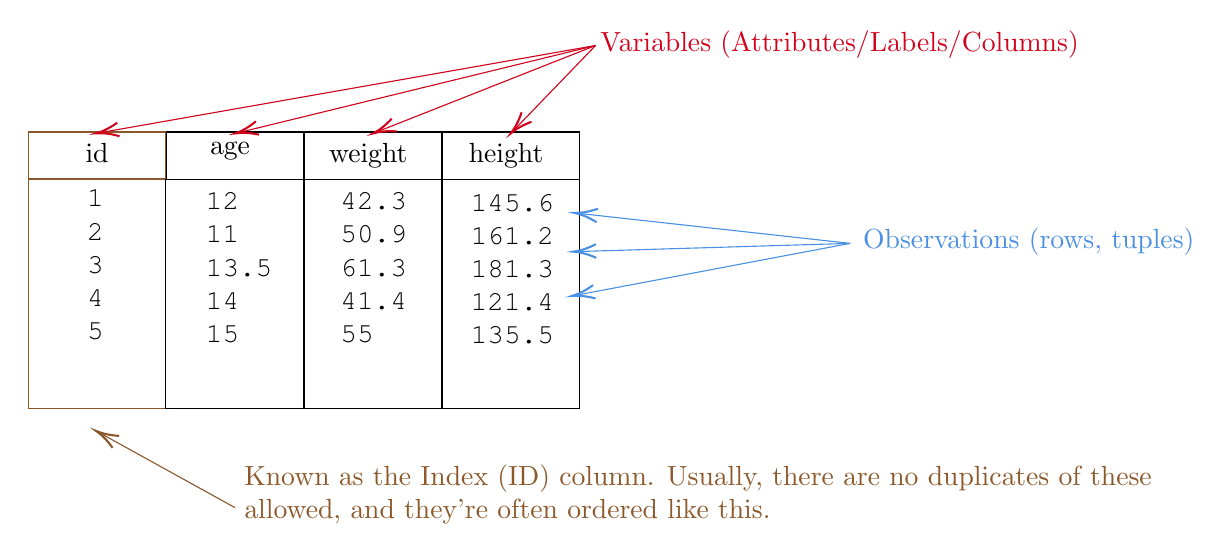
\begin{tikzpicture}[x=0.75pt,y=0.75pt,yscale=-1,xscale=1]
%uncomment if require: \path (0,300); %set diagram left start at 0, and has height of 300

%Shape: Rectangle [id:dp5949882099932227] 
\draw  [color={rgb, 255:red, 139; green, 87; blue, 42 }  ,draw opacity=1 ] (52.33,67.67) -- (118.67,67.67) -- (118.67,90.67) -- (52.33,90.67) -- cycle ;
%Shape: Rectangle [id:dp5180660849056042] 
\draw   (119,67.67) -- (185.33,67.67) -- (185.33,90.67) -- (119,90.67) -- cycle ;
%Shape: Rectangle [id:dp928756418037382] 
\draw   (185,67.67) -- (251.33,67.67) -- (251.33,90.67) -- (185,90.67) -- cycle ;
%Shape: Rectangle [id:dp982011584275448] 
\draw   (251.67,67.67) -- (318,67.67) -- (318,90.67) -- (251.67,90.67) -- cycle ;
%Shape: Rectangle [id:dp4812611593055496] 
\draw  [color={rgb, 255:red, 139; green, 87; blue, 42 }  ,draw opacity=1 ] (52.33,90.33) -- (118.67,90.33) -- (118.67,200.67) -- (52.33,200.67) -- cycle ;
%Shape: Rectangle [id:dp14867838676065692] 
\draw   (118.67,90.67) -- (185,90.67) -- (185,200.67) -- (118.67,200.67) -- cycle ;
%Shape: Rectangle [id:dp7944164207923816] 
\draw   (185.33,90.67) -- (251.67,90.67) -- (251.67,200.67) -- (185.33,200.67) -- cycle ;
%Shape: Rectangle [id:dp6914540924812163] 
\draw   (251.67,90.67) -- (318,90.67) -- (318,200.67) -- (251.67,200.67) -- cycle ;
%Straight Lines [id:da8659955223770235] 
\draw [color={rgb, 255:red, 208; green, 2; blue, 27 }  ,draw opacity=1 ]   (325.67,26) -- (86.97,67.99) ;
\draw [shift={(85,68.33)}, rotate = 350.02] [color={rgb, 255:red, 208; green, 2; blue, 27 }  ,draw opacity=1 ][line width=0.75]    (10.93,-3.29) .. controls (6.95,-1.4) and (3.31,-0.3) .. (0,0) .. controls (3.31,0.3) and (6.95,1.4) .. (10.93,3.29)   ;
%Straight Lines [id:da7649126412714919] 
\draw [color={rgb, 255:red, 208; green, 2; blue, 27 }  ,draw opacity=1 ]   (325.67,26) -- (154.11,67.86) ;
\draw [shift={(152.17,68.33)}, rotate = 346.28999999999996] [color={rgb, 255:red, 208; green, 2; blue, 27 }  ,draw opacity=1 ][line width=0.75]    (10.93,-3.29) .. controls (6.95,-1.4) and (3.31,-0.3) .. (0,0) .. controls (3.31,0.3) and (6.95,1.4) .. (10.93,3.29)   ;
%Straight Lines [id:da04591151144441219] 
\draw [color={rgb, 255:red, 208; green, 2; blue, 27 }  ,draw opacity=1 ]   (325.67,26) -- (220.36,67.6) ;
\draw [shift={(218.5,68.33)}, rotate = 338.44] [color={rgb, 255:red, 208; green, 2; blue, 27 }  ,draw opacity=1 ][line width=0.75]    (10.93,-3.29) .. controls (6.95,-1.4) and (3.31,-0.3) .. (0,0) .. controls (3.31,0.3) and (6.95,1.4) .. (10.93,3.29)   ;
%Straight Lines [id:da1253621546988095] 
\draw [color={rgb, 255:red, 208; green, 2; blue, 27 }  ,draw opacity=1 ]   (325.67,26) -- (286.22,66.89) ;
\draw [shift={(284.83,68.33)}, rotate = 313.97] [color={rgb, 255:red, 208; green, 2; blue, 27 }  ,draw opacity=1 ][line width=0.75]    (10.93,-3.29) .. controls (6.95,-1.4) and (3.31,-0.3) .. (0,0) .. controls (3.31,0.3) and (6.95,1.4) .. (10.93,3.29)   ;
%Straight Lines [id:da7853774637498458] 
\draw [color={rgb, 255:red, 74; green, 144; blue, 226 }  ,draw opacity=1 ]   (448.33,121.33) -- (317.65,106.89) ;
\draw [shift={(315.67,106.67)}, rotate = 366.31] [color={rgb, 255:red, 74; green, 144; blue, 226 }  ,draw opacity=1 ][line width=0.75]    (10.93,-3.29) .. controls (6.95,-1.4) and (3.31,-0.3) .. (0,0) .. controls (3.31,0.3) and (6.95,1.4) .. (10.93,3.29)   ;
%Straight Lines [id:da2813931715021274] 
\draw [color={rgb, 255:red, 74; green, 144; blue, 226 }  ,draw opacity=1 ]   (448.33,121.33) -- (317,125.27) ;
\draw [shift={(315,125.33)}, rotate = 358.28] [color={rgb, 255:red, 74; green, 144; blue, 226 }  ,draw opacity=1 ][line width=0.75]    (10.93,-3.29) .. controls (6.95,-1.4) and (3.31,-0.3) .. (0,0) .. controls (3.31,0.3) and (6.95,1.4) .. (10.93,3.29)   ;
%Straight Lines [id:da28293623689911906] 
\draw [color={rgb, 255:red, 74; green, 144; blue, 226 }  ,draw opacity=1 ]   (448.33,121.33) -- (316.3,146.3) ;
\draw [shift={(314.33,146.67)}, rotate = 349.28999999999996] [color={rgb, 255:red, 74; green, 144; blue, 226 }  ,draw opacity=1 ][line width=0.75]    (10.93,-3.29) .. controls (6.95,-1.4) and (3.31,-0.3) .. (0,0) .. controls (3.31,0.3) and (6.95,1.4) .. (10.93,3.29)   ;
%Straight Lines [id:da8467882522352468] 
\draw [color={rgb, 255:red, 139; green, 87; blue, 42 }  ,draw opacity=1 ]   (152,248.67) -- (86.75,212.63) ;
\draw [shift={(85,211.67)}, rotate = 388.90999999999997] [color={rgb, 255:red, 139; green, 87; blue, 42 }  ,draw opacity=1 ][line width=0.75]    (10.93,-3.29) .. controls (6.95,-1.4) and (3.31,-0.3) .. (0,0) .. controls (3.31,0.3) and (6.95,1.4) .. (10.93,3.29)   ;

% Text Node
\draw (78.67,71.67) node [anchor=north west][inner sep=0.75pt]   [align=left] {id};
% Text Node
\draw (79.5,94.33) node [anchor=north west][inner sep=0.75pt]   [align=left] {{\fontfamily{pcr}\selectfont 1}\\{\fontfamily{pcr}\selectfont 2}\\{\fontfamily{pcr}\selectfont 3}\\{\fontfamily{pcr}\selectfont 4}\\{\fontfamily{pcr}\selectfont 5}};
% Text Node
\draw (138.67,71.67) node [anchor=north west][inner sep=0.75pt]   [align=left] {age};
% Text Node
\draw (196,71.67) node [anchor=north west][inner sep=0.75pt]   [align=left] {weight};
% Text Node
\draw (263.33,71.67) node [anchor=north west][inner sep=0.75pt]   [align=left] {height};
% Text Node
\draw (136.67,95.67) node [anchor=north west][inner sep=0.75pt]   [align=left] {{\fontfamily{pcr}\selectfont 12}\\{\fontfamily{pcr}\selectfont 11}\\{\fontfamily{pcr}\selectfont 13.5}\\{\fontfamily{pcr}\selectfont 14}\\{\fontfamily{pcr}\selectfont 15}};
% Text Node
\draw (201.5,95.67) node [anchor=north west][inner sep=0.75pt]   [align=left] {{\fontfamily{pcr}\selectfont 42.3}\\{\fontfamily{pcr}\selectfont 50.9}\\{\fontfamily{pcr}\selectfont 61.3}\\{\fontfamily{pcr}\selectfont 41.4}\\{\fontfamily{pcr}\selectfont 55}};
% Text Node
\draw (264.33,96.33) node [anchor=north west][inner sep=0.75pt]   [align=left] {{\fontfamily{pcr}\selectfont 145.6}\\{\fontfamily{pcr}\selectfont 161.2}\\{\fontfamily{pcr}\selectfont 181.3}\\{\fontfamily{pcr}\selectfont 121.4}\\{\fontfamily{pcr}\selectfont 135.5}};
% Text Node
\draw (326.67,17.67) node [anchor=north west][inner sep=0.75pt]   [align=left] {\textcolor[rgb]{0.82,0.01,0.11}{Variables (Attributes/Labels/Columns)}};
% Text Node
\draw (453.33,112.33) node [anchor=north west][inner sep=0.75pt]   [align=left] {\textcolor[rgb]{0.29,0.56,0.89}{Observations (rows, tuples)}};
% Text Node
\draw (155.17,226.67) node [anchor=north west][inner sep=0.75pt]   [align=left] {\textcolor[rgb]{0.55,0.34,0.16}{Known as the Index (ID) column. Usually, there are no duplicates of these}\\\textcolor[rgb]{0.55,0.34,0.16}{allowed, and they're often ordered like this.}};


\end{tikzpicture}

}


\hfill \break Here's an example table. I've highlighted and color coded the important aspects of it. Remember, don't think of this as the data structure itself- this is just an abstraction to help us keep track of our vast amounts of data. However, most table implementations do a pretty good job of representing the stuff I've color coded.\\

\subsubsection{Selecting / Slicing}

Selecting one or more of the rows or columns in particular to analyze. Examples:

\begin{itemize}
	\item Select only columns ID + Age
	\item Select all rows with weight > 41
	\item We can also apply a combination of the above 2. (\textit{You can combine select rules!})
\end{itemize}

\subsubsection{Aggregating / Reducing}

Combining values across a column into a single value. (We don't do this across rows, because that obviously wouldn't make any sense. Think about it!). Examples:

\begin{itemize}
	\item Find the sum of all row's columns
	\item Find the max of the weight column
\end{itemize}

\textbf{Note:} It's usually never useful to aggregate/reduce the ID column, so for most cases, we ignore it when we perform such operations.

\subsubsection{Map}

Apply a function to every row, possibly creating fewer or more columns. This one's a little weird to think about without a clear example, so I'm including one below.\\

{
\centering



\tikzset{every picture/.style={line width=0.75pt}} %set default line width to 0.75pt        

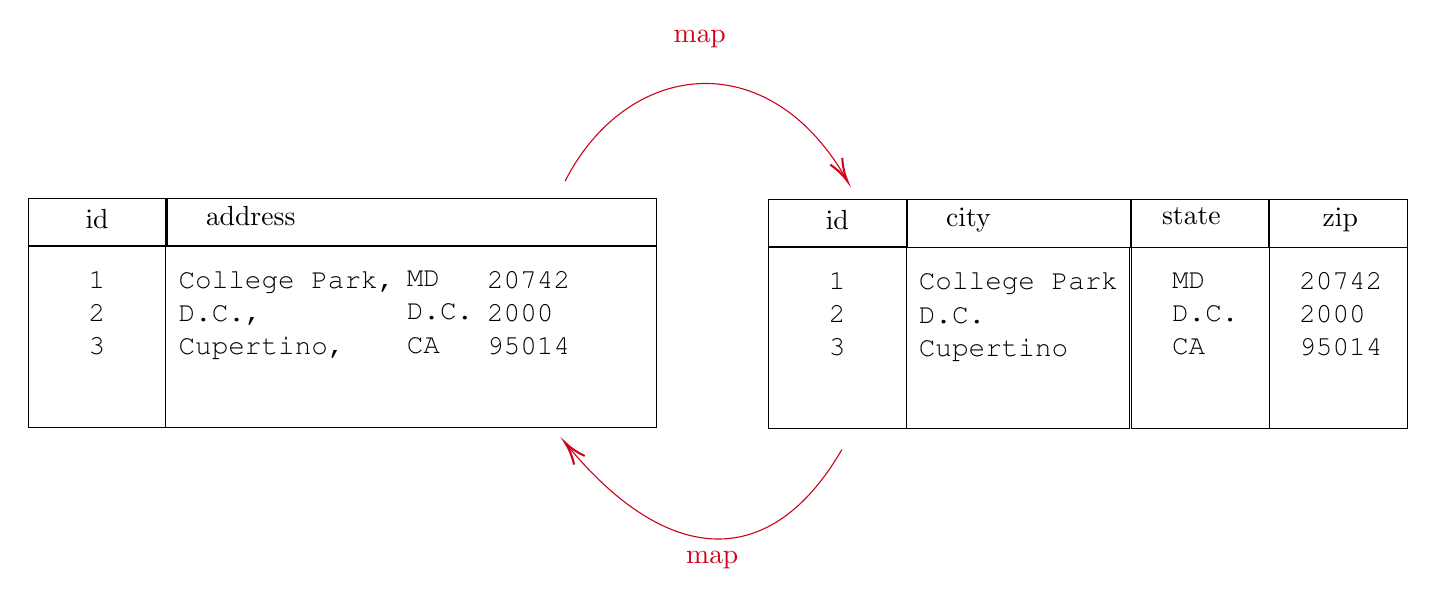
\begin{tikzpicture}[x=0.75pt,y=0.75pt,yscale=-1,xscale=1]
%uncomment if require: \path (0,300); %set diagram left start at 0, and has height of 300

%Shape: Rectangle [id:dp4887463946097159] 
\draw  [color={rgb, 255:red, 0; green, 0; blue, 0 }  ,draw opacity=1 ] (362.33,88.33) -- (428.67,88.33) -- (428.67,111.33) -- (362.33,111.33) -- cycle ;
%Shape: Rectangle [id:dp5770783881644757] 
\draw  [color={rgb, 255:red, 0; green, 0; blue, 0 }  ,draw opacity=1 ] (429.21,88.33) -- (537,88.33) -- (537,111.33) -- (429.21,111.33) -- cycle ;
%Shape: Rectangle [id:dp6134551110117208] 
\draw   (537,88.33) -- (603.33,88.33) -- (603.33,111.33) -- (537,111.33) -- cycle ;
%Shape: Rectangle [id:dp5531077995700737] 
\draw   (603.67,88.33) -- (670,88.33) -- (670,111.33) -- (603.67,111.33) -- cycle ;
%Shape: Rectangle [id:dp3313757499092773] 
\draw  [color={rgb, 255:red, 0; green, 0; blue, 0 }  ,draw opacity=1 ] (362.33,111) -- (428.67,111) -- (428.67,198.67) -- (362.33,198.67) -- cycle ;
%Shape: Rectangle [id:dp9339502110856537] 
\draw  [color={rgb, 255:red, 0; green, 0; blue, 0 }  ,draw opacity=1 ] (428.67,111.26) -- (536.46,111.26) -- (536.46,198.67) -- (428.67,198.67) -- cycle ;
%Shape: Rectangle [id:dp07892533389980638] 
\draw   (537.33,111.26) -- (603.67,111.26) -- (603.67,198.67) -- (537.33,198.67) -- cycle ;
%Shape: Rectangle [id:dp979611278461765] 
\draw   (603.67,111.26) -- (670,111.26) -- (670,198.67) -- (603.67,198.67) -- cycle ;
%Shape: Rectangle [id:dp717440949324254] 
\draw  [color={rgb, 255:red, 0; green, 0; blue, 0 }  ,draw opacity=1 ] (5.67,87.67) -- (72,87.67) -- (72,110.67) -- (5.67,110.67) -- cycle ;
%Shape: Rectangle [id:dp5659022269665408] 
\draw  [color={rgb, 255:red, 0; green, 0; blue, 0 }  ,draw opacity=1 ] (72.54,87.67) -- (308.33,87.67) -- (308.33,110.67) -- (72.54,110.67) -- cycle ;
%Shape: Rectangle [id:dp9470998578275607] 
\draw  [color={rgb, 255:red, 0; green, 0; blue, 0 }  ,draw opacity=1 ] (5.67,110.33) -- (72,110.33) -- (72,198) -- (5.67,198) -- cycle ;
%Shape: Rectangle [id:dp5421589353414771] 
\draw  [color={rgb, 255:red, 0; green, 0; blue, 0 }  ,draw opacity=1 ] (72,110.6) -- (308.33,110.6) -- (308.33,198) -- (72,198) -- cycle ;
%Curve Lines [id:da1781160675260307] 
\draw [color={rgb, 255:red, 208; green, 2; blue, 27 }  ,draw opacity=1 ]   (264.33,79.33) .. controls (294.18,20.96) and (362.31,12.75) .. (399.77,78.34) ;
\draw [shift={(400.33,79.33)}, rotate = 240.75] [color={rgb, 255:red, 208; green, 2; blue, 27 }  ,draw opacity=1 ][line width=0.75]    (10.93,-3.29) .. controls (6.95,-1.4) and (3.31,-0.3) .. (0,0) .. controls (3.31,0.3) and (6.95,1.4) .. (10.93,3.29)   ;
%Curve Lines [id:da028217104849822316] 
\draw [color={rgb, 255:red, 208; green, 2; blue, 27 }  ,draw opacity=1 ]   (397.67,208.67) .. controls (363.84,267.04) and (314.17,266.01) .. (265.07,206.24) ;
\draw [shift={(264.33,205.33)}, rotate = 410.88] [color={rgb, 255:red, 208; green, 2; blue, 27 }  ,draw opacity=1 ][line width=0.75]    (10.93,-3.29) .. controls (6.95,-1.4) and (3.31,-0.3) .. (0,0) .. controls (3.31,0.3) and (6.95,1.4) .. (10.93,3.29)   ;

% Text Node
\draw (388.67,92.33) node [anchor=north west][inner sep=0.75pt]   [align=left] {id};
% Text Node
\draw (390.17,122.06) node [anchor=north west][inner sep=0.75pt]   [align=left] {{\fontfamily{pcr}\selectfont 1}\\{\fontfamily{pcr}\selectfont 2}\\{\fontfamily{pcr}\selectfont 3}};
% Text Node
\draw (446.67,91) node [anchor=north west][inner sep=0.75pt]   [align=left] {city};
% Text Node
\draw (550.67,91) node [anchor=north west][inner sep=0.75pt]   [align=left] {state};
% Text Node
\draw (628,91) node [anchor=north west][inner sep=0.75pt]   [align=left] {zip};
% Text Node
\draw (433.5,122.06) node [anchor=north west][inner sep=0.75pt]   [align=left] {{\fontfamily{pcr}\selectfont College Park}\\{\fontfamily{pcr}\selectfont D.C.}\\{\fontfamily{pcr}\selectfont Cupertino}};
% Text Node
\draw (555.5,122.06) node [anchor=north west][inner sep=0.75pt]   [align=left] {{\fontfamily{pcr}\selectfont MD}\\{\fontfamily{pcr}\selectfont D.C.}\\{\fontfamily{pcr}\selectfont CA}};
% Text Node
\draw (616.83,122.06) node [anchor=north west][inner sep=0.75pt]   [align=left] {{\fontfamily{pcr}\selectfont 20742}\\{\fontfamily{pcr}\selectfont 2000}\\{\fontfamily{pcr}\selectfont 95014}};
% Text Node
\draw (32,91.67) node [anchor=north west][inner sep=0.75pt]   [align=left] {id};
% Text Node
\draw (33.5,121.39) node [anchor=north west][inner sep=0.75pt]   [align=left] {{\fontfamily{pcr}\selectfont 1}\\{\fontfamily{pcr}\selectfont 2}\\{\fontfamily{pcr}\selectfont 3}};
% Text Node
\draw (90,90.33) node [anchor=north west][inner sep=0.75pt]   [align=left] {address};
% Text Node
\draw (76.83,121.39) node [anchor=north west][inner sep=0.75pt]   [align=left] {{\fontfamily{pcr}\selectfont College Park,}\\{\fontfamily{pcr}\selectfont D.C., }\\{\fontfamily{pcr}\selectfont Cupertino, }};
% Text Node
\draw (186.83,121.39) node [anchor=north west][inner sep=0.75pt]   [align=left] {{\fontfamily{pcr}\selectfont MD}\\{\fontfamily{pcr}\selectfont D.C.}\\{\fontfamily{pcr}\selectfont CA}};
% Text Node
\draw (225.5,121.39) node [anchor=north west][inner sep=0.75pt]   [align=left] {{\fontfamily{pcr}\selectfont 20742}\\{\fontfamily{pcr}\selectfont 2000}\\{\fontfamily{pcr}\selectfont 95014}};
% Text Node
\draw (315.33,5.67) node [anchor=north west][inner sep=0.75pt]   [align=left] {\textcolor[rgb]{0.82,0.01,0.11}{map}};
% Text Node
\draw (321.33,256.33) node [anchor=north west][inner sep=0.75pt]   [align=left] {\textcolor[rgb]{0.82,0.01,0.11}{map}};


\end{tikzpicture}

}

\hfill \break Notice how applying map to either table is valid in this case- sometimes we want to break down columns into more specific values, and sometimes we want to combine them into singular columns. Each of these operations is totally valid, and has its uses. (This is evident in the projects for this class).\\

Again, this is mostly about what you need. There's no necessary better or worse in this case (more columns does not always equal better data).

\subsubsection{Group By}

Group By is an operation that allows you to group tuples together based on the values in columns/dimensions. Let's say we had the following table of house addresses like earlier. This time, we'll add the number of people in each house as a column as well.\\

{
\centering



\tikzset{every picture/.style={line width=0.75pt}} %set default line width to 0.75pt        

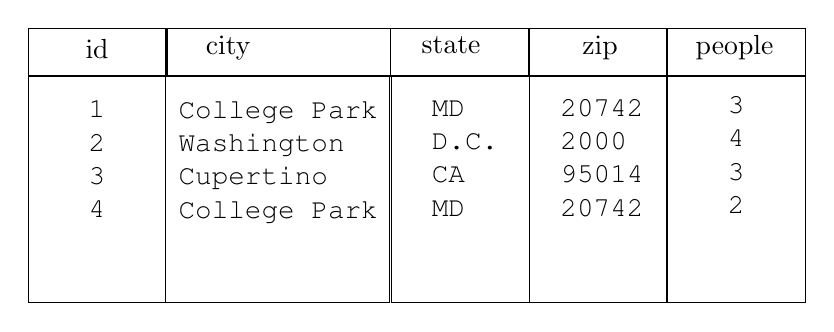
\begin{tikzpicture}[x=0.75pt,y=0.75pt,yscale=-1,xscale=1]
%uncomment if require: \path (0,300); %set diagram left start at 0, and has height of 300

%Shape: Rectangle [id:dp816510738764739] 
\draw  [color={rgb, 255:red, 0; green, 0; blue, 0 }  ,draw opacity=1 ] (185,62.33) -- (251.33,62.33) -- (251.33,85.33) -- (185,85.33) -- cycle ;
%Shape: Rectangle [id:dp39744801489204895] 
\draw  [color={rgb, 255:red, 0; green, 0; blue, 0 }  ,draw opacity=1 ] (251.87,62.33) -- (359.67,62.33) -- (359.67,85.33) -- (251.87,85.33) -- cycle ;
%Shape: Rectangle [id:dp16790194728351993] 
\draw   (359.67,62.33) -- (426,62.33) -- (426,85.33) -- (359.67,85.33) -- cycle ;
%Shape: Rectangle [id:dp5121628997613088] 
\draw   (426.33,62.33) -- (492.67,62.33) -- (492.67,85.33) -- (426.33,85.33) -- cycle ;
%Shape: Rectangle [id:dp38170728474734883] 
\draw  [color={rgb, 255:red, 0; green, 0; blue, 0 }  ,draw opacity=1 ] (185,85) -- (251.33,85) -- (251.33,194.67) -- (185,194.67) -- cycle ;
%Shape: Rectangle [id:dp0783518509199912] 
\draw  [color={rgb, 255:red, 0; green, 0; blue, 0 }  ,draw opacity=1 ] (251.33,85.33) -- (359.12,85.33) -- (359.12,194.67) -- (251.33,194.67) -- cycle ;
%Shape: Rectangle [id:dp8309347187193188] 
\draw   (360,85.33) -- (426.33,85.33) -- (426.33,194.67) -- (360,194.67) -- cycle ;
%Shape: Rectangle [id:dp0878616379496251] 
\draw   (426.33,85.33) -- (492.67,85.33) -- (492.67,194.67) -- (426.33,194.67) -- cycle ;
%Shape: Rectangle [id:dp9451653351898317] 
\draw   (493,62.33) -- (559.33,62.33) -- (559.33,85.33) -- (493,85.33) -- cycle ;
%Shape: Rectangle [id:dp11005059918565219] 
\draw   (493,85.33) -- (559.33,85.33) -- (559.33,194.67) -- (493,194.67) -- cycle ;

% Text Node
\draw (211.33,66.33) node [anchor=north west][inner sep=0.75pt]   [align=left] {id};
% Text Node
\draw (212.83,96.06) node [anchor=north west][inner sep=0.75pt]   [align=left] {{\fontfamily{pcr}\selectfont 1}\\{\fontfamily{pcr}\selectfont 2}\\{\fontfamily{pcr}\selectfont 3}\\{\fontfamily{pcr}\selectfont 4}\\};
% Text Node
\draw (269.33,65) node [anchor=north west][inner sep=0.75pt]   [align=left] {city};
% Text Node
\draw (373.33,65) node [anchor=north west][inner sep=0.75pt]   [align=left] {state};
% Text Node
\draw (450.67,65) node [anchor=north west][inner sep=0.75pt]   [align=left] {zip};
% Text Node
\draw (256.17,96.06) node [anchor=north west][inner sep=0.75pt]   [align=left] {{\fontfamily{pcr}\selectfont College Park}\\{\fontfamily{pcr}\selectfont Washington}\\{\fontfamily{pcr}\selectfont Cupertino}\\{\fontfamily{pcr}\selectfont College Park}};
% Text Node
\draw (378.17,96.06) node [anchor=north west][inner sep=0.75pt]   [align=left] {{\fontfamily{pcr}\selectfont MD}\\{\fontfamily{pcr}\selectfont D.C.}\\{\fontfamily{pcr}\selectfont CA}\\{\fontfamily{pcr}\selectfont MD}};
% Text Node
\draw (440.17,95.39) node [anchor=north west][inner sep=0.75pt]   [align=left] {{\fontfamily{pcr}\selectfont 20742}\\{\fontfamily{pcr}\selectfont 2000}\\{\fontfamily{pcr}\selectfont 95014}\\{\fontfamily{pcr}\selectfont 20742}};
% Text Node
\draw (505.33,64.33) node [anchor=north west][inner sep=0.75pt]   [align=left] {people};
% Text Node
\draw (520.83,94.06) node [anchor=north west][inner sep=0.75pt]   [align=left] {{\fontfamily{pcr}\selectfont 3}\\{\fontfamily{pcr}\selectfont 4}\\{\fontfamily{pcr}\selectfont 3}\\{\fontfamily{pcr}\selectfont 2}};


\end{tikzpicture}

}

Let's say we only wanted to see the data from a \textbf{single city}. In this case, let's pick College Park.\newline

{
\centering



\tikzset{every picture/.style={line width=0.75pt}} %set default line width to 0.75pt        

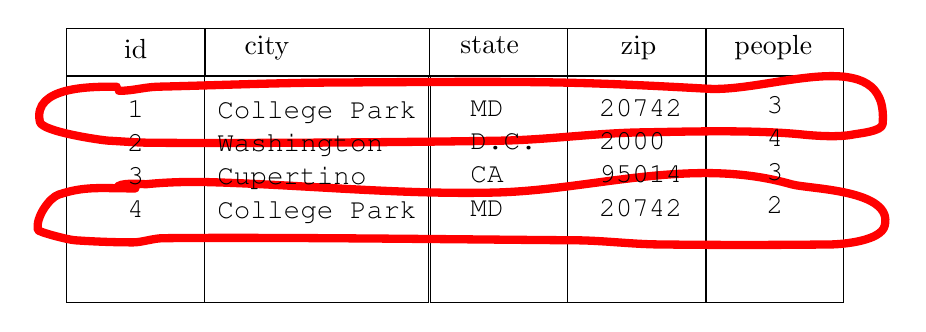
\begin{tikzpicture}[x=0.75pt,y=0.75pt,yscale=-1,xscale=1]
%uncomment if require: \path (0,300); %set diagram left start at 0, and has height of 300

%Shape: Rectangle [id:dp816510738764739] 
\draw  [color={rgb, 255:red, 0; green, 0; blue, 0 }  ,draw opacity=1 ] (185,62.33) -- (251.33,62.33) -- (251.33,85.33) -- (185,85.33) -- cycle ;
%Shape: Rectangle [id:dp39744801489204895] 
\draw  [color={rgb, 255:red, 0; green, 0; blue, 0 }  ,draw opacity=1 ] (251.87,62.33) -- (359.67,62.33) -- (359.67,85.33) -- (251.87,85.33) -- cycle ;
%Shape: Rectangle [id:dp16790194728351993] 
\draw   (359.67,62.33) -- (426,62.33) -- (426,85.33) -- (359.67,85.33) -- cycle ;
%Shape: Rectangle [id:dp5121628997613088] 
\draw   (426.33,62.33) -- (492.67,62.33) -- (492.67,85.33) -- (426.33,85.33) -- cycle ;
%Shape: Rectangle [id:dp38170728474734883] 
\draw  [color={rgb, 255:red, 0; green, 0; blue, 0 }  ,draw opacity=1 ] (185,85) -- (251.33,85) -- (251.33,194.67) -- (185,194.67) -- cycle ;
%Shape: Rectangle [id:dp0783518509199912] 
\draw  [color={rgb, 255:red, 0; green, 0; blue, 0 }  ,draw opacity=1 ] (251.33,85.33) -- (359.12,85.33) -- (359.12,194.67) -- (251.33,194.67) -- cycle ;
%Shape: Rectangle [id:dp8309347187193188] 
\draw   (360,85.33) -- (426.33,85.33) -- (426.33,194.67) -- (360,194.67) -- cycle ;
%Shape: Rectangle [id:dp0878616379496251] 
\draw   (426.33,85.33) -- (492.67,85.33) -- (492.67,194.67) -- (426.33,194.67) -- cycle ;
%Shape: Rectangle [id:dp9451653351898317] 
\draw   (493,62.33) -- (559.33,62.33) -- (559.33,85.33) -- (493,85.33) -- cycle ;
%Shape: Rectangle [id:dp11005059918565219] 
\draw   (493,85.33) -- (559.33,85.33) -- (559.33,194.67) -- (493,194.67) -- cycle ;
%Shape: Free Drawing [id:dp983490163154191] 
\draw  [color={rgb, 255:red, 255; green, 0; blue, 0 }  ,draw opacity=1 ][line width=3] [line join = round][line cap = round] (209,90.5) .. controls (198.12,90.5) and (168.09,89.91) .. (172,107.5) .. controls (173.05,112.21) and (201.95,116.35) .. (205,116.5) .. controls (211.67,116.83) and (218.33,117.44) .. (225,117.5) .. controls (265.32,117.85) and (345.68,117.33) .. (394,116.5) .. controls (416.57,116.11) and (439.52,112.83) .. (462,112.5) .. controls (480.28,112.24) and (514.78,111.08) .. (539,113.5) .. controls (546.8,114.28) and (556.96,114.91) .. (564,113.5) .. controls (566.72,112.96) and (577.71,112.02) .. (578,108.5) .. controls (581.35,68.27) and (524.35,93.19) .. (494,91.5) .. controls (427.64,87.81) and (413.09,87.87) .. (312,88.5) .. controls (284.83,88.67) and (256.23,89.85) .. (229,90.5) .. controls (222.28,90.66) and (216.95,92.5) .. (210,92.5) ;
%Curve Lines [id:da10861026576502275] 
\draw [color={rgb, 255:red, 255; green, 0; blue, 0 }  ,draw opacity=1 ][line width=3] [line join = round][line cap = round]   (218,139.5) .. controls (201.04,139.5) and (193.69,138.27) .. (181,142.5) .. controls (176.53,143.99) and (169.8,153.48) .. (171,159.5) .. controls (171.2,160.48) and (185.36,164.26) .. (189,164.5) .. controls (198.32,165.12) and (207.66,165.5) .. (217,165.5) .. controls (221.09,165.5) and (226.66,163.55) .. (231,163.5) .. controls (282.82,162.87) and (384.95,164.21) .. (430,164.5) .. controls (443.35,164.59) and (456.65,166.35) .. (470,166.5) .. controls (497.66,166.82) and (525.34,166.82) .. (553,166.5) .. controls (558.97,166.43) and (577.17,164.8) .. (579,157.5) .. controls (583.4,139.91) and (542.58,139.95) .. (534,137.5) .. controls (486.11,123.82) and (438.47,140.4) .. (391,141.5) .. controls (345.12,142.57) and (299.53,137.8) .. (254,136.5) .. controls (243.67,136.2) and (233.29,136.47) .. (223,137.5) .. controls (222.9,137.51) and (209,136.14) .. (209,139.5) ;

% Text Node
\draw (211.33,66.33) node [anchor=north west][inner sep=0.75pt]   [align=left] {id};
% Text Node
\draw (212.83,96.06) node [anchor=north west][inner sep=0.75pt]   [align=left] {{\fontfamily{pcr}\selectfont 1}\\{\fontfamily{pcr}\selectfont 2}\\{\fontfamily{pcr}\selectfont 3}\\{\fontfamily{pcr}\selectfont 4}\\};
% Text Node
\draw (269.33,65) node [anchor=north west][inner sep=0.75pt]   [align=left] {city};
% Text Node
\draw (373.33,65) node [anchor=north west][inner sep=0.75pt]   [align=left] {state};
% Text Node
\draw (450.67,65) node [anchor=north west][inner sep=0.75pt]   [align=left] {zip};
% Text Node
\draw (256.17,96.06) node [anchor=north west][inner sep=0.75pt]   [align=left] {{\fontfamily{pcr}\selectfont College Park}\\{\fontfamily{pcr}\selectfont Washington}\\{\fontfamily{pcr}\selectfont Cupertino}\\{\fontfamily{pcr}\selectfont College Park}};
% Text Node
\draw (378.17,96.06) node [anchor=north west][inner sep=0.75pt]   [align=left] {{\fontfamily{pcr}\selectfont MD}\\{\fontfamily{pcr}\selectfont D.C.}\\{\fontfamily{pcr}\selectfont CA}\\{\fontfamily{pcr}\selectfont MD}};
% Text Node
\draw (440.17,95.39) node [anchor=north west][inner sep=0.75pt]   [align=left] {{\fontfamily{pcr}\selectfont 20742}\\{\fontfamily{pcr}\selectfont 2000}\\{\fontfamily{pcr}\selectfont 95014}\\{\fontfamily{pcr}\selectfont 20742}};
% Text Node
\draw (505.33,64.33) node [anchor=north west][inner sep=0.75pt]   [align=left] {people};
% Text Node
\draw (520.83,94.06) node [anchor=north west][inner sep=0.75pt]   [align=left] {{\fontfamily{pcr}\selectfont 3}\\{\fontfamily{pcr}\selectfont 4}\\{\fontfamily{pcr}\selectfont 3}\\{\fontfamily{pcr}\selectfont 2}};


\end{tikzpicture}

}

This is what a 'Group By' operation would be perfect for. It'll basically just get us the rows that are from the city that we want.

\subsubsection{Group By + Aggregate}

We can combined Group By and Aggregate in pretty cool ways to get results that we want. For example, let's say we wanted to leverage the above table and get the sum total of all people who live in College Park, D.C., and Cupertino, respectively. By using a combo of Group By and Aggregate, we can totally do that. (\textit{Group By} City, then perform summing \textit{aggregation} operation.)

\subsubsection{Union, Intersection, Difference}

These are your usual set operations from statistics. However, this only works if the tables have identical attributes (columns). If they have identical columns, they are called \textbf{compatible tables}.\\

Examples: (Table A) $\union$ (Table B) results in (Table C) where all three tables have the same attributes. Likewise, (Table A) $\cap$ (Table B) results in (Table D) where all three also have the same attributes.

\section{Footnotes}

Taken by Akilesh Praveen.

\end{document}
